% Multiple Choice Question 25 to 26 (2 questions)

% \par\noindent\rule{0.75\textwidth}{0.5pt} 
\textbf{See the instruction for questions \inteval{\value{question}+1} to \inteval{\value{question}+2}.} 

\begin{center}
    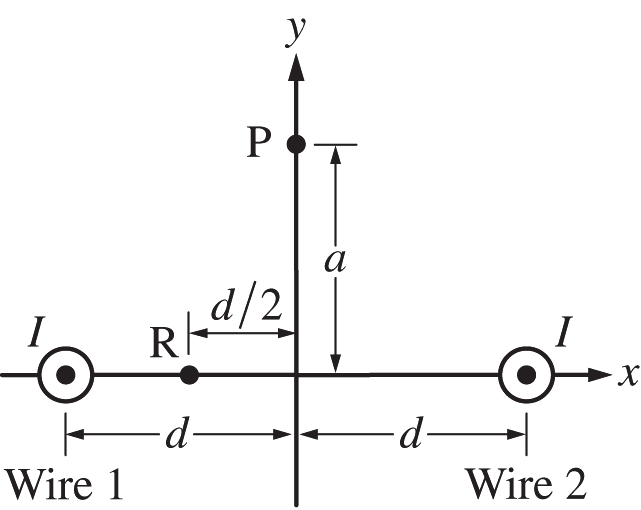
\includegraphics[scale=0.3]{images/img-012-019.png}
\end{center}

Two wires perpendicular to the $x$-axis have currents $I$ directed out of the page, as shown above. Each wire is a distance $d$ from the $y$-axis. Point P lies on the $y$-axis at the coordinate $(0, a)$, and point R lies on the $x$-axis at the coordinate $(-d / 2,0)$.

\begin{questions}
\setcounter{question}{24}

% Multiple Choice Question 25
\question
Which of the following expressions represents the magnitude of the magnetic field at point R?

\begin{oneparchoices}
    \choice Zero
    \choice $\dfrac{\mu_{0} I}{2 \pi d}$ 
    \choice $\dfrac{\mu_{0} I}{\pi d}$ 
    \choice $\dfrac{4 \mu_{0} I}{3 \pi d}$ 
    \choice $\dfrac{2 \mu_{0} I}{3 \pi d}$
\end{oneparchoices}

% Multiple Choice Question 26
\question
Which of the following best represents the direction of the net magnetic field at point P?

\begin{oneparchoices}
    \choice \adjustbox{valign=t}{
\includegraphics[scale=0.2]{images/img-012-020.png}}
    \choice \adjustbox{valign=t}{
\includegraphics[scale=0.2]{images/img-012-021.png}}
    \choice \adjustbox{valign=t}{
\includegraphics[scale=0.2]{images/img-012-022.png}}
    \choice \adjustbox{valign=t}{
\includegraphics[scale=0.2]{images/img-012-023.png}}
    \choice \adjustbox{valign=t}{
\includegraphics[scale=0.2]{images/img-012-024.png}}
\end{oneparchoices}

\end{questions}
